\chapter{SEPARATION AXIOMS}\label{chp:2_1_2}

\section{Four separation axioms}

By "separation axioms" we mean properties of topological spaces concerning separating certain disjoint sets via (disjoint) open sets. [Caution: It is very different from
the conception separable that we learned last time!] There are many different separations axioms 1
, four of them are used more often than the others, and we have seen
two of them which are most important:


\begin{definition}{}{}
    ($T_1$)
    \begin{align*}
        \forall x_1\neq x_2\in X,\exists \text{ open sets }U,K \text{ s.t. }\\
        x_1\in U\text{ but } x_2\notin U \text{ and } x_2\in K\text{ but } x_1\notin K. 
    \end{align*}
    ($T_2$)
    \begin{align*}
        \forall x_1\neq x_2\in X,\exists \text{ open sets } U,K \text{ s.t. }\\
        x_1\in U,x_2\in K \text{ and }U\cap K=\O.
    \end{align*}
    ($T_3$)
    \begin{align*}
        \forall \text{ closed sets }V \text{ and }x\notin V, \exists \text{ open sets } U,K \text{ s.t. }\\
        V\subset U, x\in K \text{ and } U\cap K=\O.
    \end{align*}
    ($T_4$)
    \begin{align*}
        \forall \text{ closed sets } V_1 \text{ and } V_2 \text{ with } V_1\cap V_2=\O, \exists \text{ open sets }\\
        U,K \text{ s.t. } V_1\subset U, V_2\subset K \text{ and }U\cap K=\O.
    \end{align*}
\end{definition}

\begin{figure}[htbp]
    \centering
    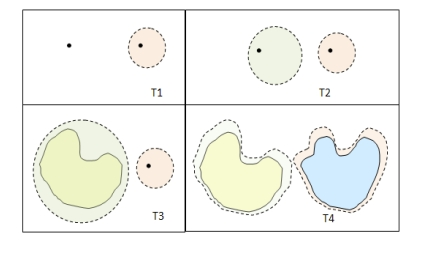
\includegraphics[width=0.6\textwidth]{figure/separation/separation_fig.png}
    \caption{}
\end{figure}

\begin{remark}
    In some books, "both (T1) and (T3)" in our sense means "regular" 
    "both (T1) and (T4)" means "normal"; in some other books, "(T3)" means "regular"
    and "(T4)" means "normal". In order to reduce ambiguity, we only talk about (T1-T4) in our sense
    but not "regular" and "normal". 

\end{remark}

\section{Equivalent characterizations}
First we give equivalent characterizations of these axioms.
\begin{proposition}{}{}
    Let $(X,\tau)$ be a topological space.\\
    (1) $(X,\tau)$ is (T1) iff any single point set is closed.\\
    (2) $(X,\tau)$ is (T2) iff the diagonal $\triangle =\{(x,x):x\in X\}$ is closed in $X\times X$.\\
    (3) $(X,\tau)$ is (T3) iff $\forall$ open set $U$ with $x\in U$, $\exists \text{ open set } K$ such that $x\in K\subset \overline{K}\subset U$\\
    (4) $(X,\tau)$ is (T4) iff $\forall$ closed set $V\subset U$($U$ is open), $\exists \text{ open set }K$ such that $V\subset K\subset \overline{K}\subset U$.
\end{proposition}

\begin{proof}
    (1) and (2) follow from definitions, while (3) and (4)
follow from open-closed duality:\\
(1) ($\Rightarrow$): For $\forall y\neq x$, $\exists U_y\in \tau$ such that $y\in U_y$ but $x\notin U$, then $U_y\subset \{x\}^c$ 
    and $\{x\}^c=\cup_{y\neq x}U_y$.
    is open, i.e. $\{x\}$ is closed. \\
    ($\Leftarrow$): For $\forall x\neq y$, take $U={y}^c$ and $K={x}^c$. Then $U,K$ is open and $x\in U, y\in K$ but $x\notin K, y\notin U$.\\
(2) The proof is trivial if $|X|=1$, assume that $|X|>1$.\\
    ($\Rightarrow$): 
    Suppose $X$ is Hausdorff. Let $(a,b)\in X\times X-\triangle$. 
    (Note that such an element exists, since $|X|>1$). Then, $a\neq b$.
    Since $X$ is Hausdorff, we can pick open sets $U_a$ and $U_b$ such that $a\in U_a,b\in U_b$ and $U_a\cap U_b=\O$.
    Now, note that $(U_a\times U_b)\cap \triangle = \O$ (If not, $\exists (p,q)\in (U_a\times U_b)\cap \triangle$. 
    Then $(p,q)\in \triangle$ and so $p=q$. But then $p\in U_a$ and $p\in U_b$, contradicting the fact that $U_a\cap U_b=\O$.)
    Since $U_a\times U_b\in \tau_{X\times X}$ and $(a,b)\in U_a\times U_b\subseteq X\times X-\triangle$, 
    by proposition\ref{prop:open set judging}, $X\times X-\triangle$ is open in $X\times X$. 
    Hence, $\triangle$ is closed in $X\times X$.\\
    ($\Leftarrow$): For $x\neq y\in X$, i.e. $(x,y)\in \triangle^c$, there exists $U,K$ such that $x\in U,y\in K$ and
    $(x,y)\in U\times K\subseteq \triangle^c$. 
    It follows $U\cap K=\O$, if not, there exists $z\in U\cap K$, 
    then $(z,z)\in U\times K\cap\triangle=\O$. This is a contradiction. 
    Hence, $X$ is Hausdorff.\\
(3) ($\Rightarrow$):
    $\forall$ open set $U$ with $x\in U$, then $x\notin U^c$ (closed set).
    Then, there exists $K_1,K_2\in \tau$ such that $x\in K_1, U^c\subset K_2$ and $K_1\cap K_2=\O$.
    Then by proposition\ref{prop:closure and interior relation}, $x\in K_1\subset \overline{K_1}\subset K_2^c\subset U$.\\
    ($\Leftarrow$):
    Suppose $x\notin V$ closed, i.e. $x\in V^c$ open, then there exists $K\in \tau$ such that 
    $x\in K\subset \overline{K}\subset V^c$. It follows $K\cap \overline{K}^c=\O$, $x\in K$ and $V\subset \overline{K}^c$.\\
(4) ($\Rightarrow$):
    Suppose closed $V\subset U$ open, then $V\cap U^c=\O$.
    So there exists $K_1,K_2\in\tau$ such that $K_1\cap K_2=\O, V\subset K_1$ and $U^c\subset K_2$.
    So $V\subset K_1\subset \overline{K_1}\subset K_2^c\subset U$.\\
    ($\Leftarrow$):
    Suppose $V_1,V_2$ are closed and $V_1\cap V_2=\O$. Then $V_1\subset V_2^c$ open. 
    So there exists $K\in \tau$ such that $V\subset K\subset \overline{K}\subset V_2^c$.
    It follows that $K\cap \overline{K}^c=\O$, $V\subset K$ and $V_2\subset \overline{K}^c$. 
\end{proof}


\section{Relations between different separation axioms}


We can also study the relations between these axioms. Obviously we have
\begin{proposition}{}{}
    (1) $T_2\Rightarrow T_1$.\\
    (2) $T_1+T_3\Rightarrow T_2, T_1+T_4\Rightarrow T_2, T_1+T_4\Rightarrow T_3$.\\
\end{proposition}

\begin{proof}
    (1) \begin{align*}
    \forall x_1\neq x_2\in X &\overset{T2}{\Rightarrow} \exists U,K\in \tau: x_1\in U,x_2\in K \text{ and } U\cap K=\O\\
                            & \Rightarrow x_1\in U, x\notin K \text{ and } x_2\in K, x_2\notin U\\
                            & \Rightarrow x_1\in U\setminus K \text{ and } x_2\in K\setminus U.
        \end{align*}
    (2) 
    \begin{align*}
        \forall x_1\neq x_2\in X &\overset{T1}{\Rightarrow} \{x_1\} \text{ is closed and } x_2\notin \{x_1\}\\
                                & \overset{T3}{\Rightarrow} \exists U,K\in \tau \text{ s.t. } \{x_1\}\subseteq U, x_2\in K \text{ and } U\cap K=\O.\\
                                & \Rightarrow x_1\in U,x_2\in K \text{ and } U\cap K=\O.
    \end{align*}
    \begin{align*}
        1
    \end{align*}
\end{proof}

\begin{proposition}{}{}
    A metric sapce satisfys $T_1,T_2,T_3 \text{ and } T_4$.
\end{proposition}

\section{Productive and hereditary}

\begin{proposition}{}{}
    $T_1$ is hereditary. 
\end{proposition}

\begin{proof}
    Let $(X,\tau)$ be a $T_1$ space and $A\subset X$. That is: 
    \begin{align*}
        \forall x\neq y\in A\subset X, \exists U,K\in\tau:\\
        x\in U\text{ but } y\notin U\text{ and } y\in K\text{ but } x\notin K.
    \end{align*}
    Then one can find
    \begin{align*}
        U_A := U\cap A, K_A:=K\cap A.
    \end{align*}
    It follows that $U_A,K_A\in \tau_A$ s.t. $x\in U_A$ but $y\notin U_A$ and $y\in K_A$ but $x\notin K_A$
\end{proof}


\begin{proposition}{}{}
    $T_2$ is hereditary. 
\end{proposition}

\begin{proof}
    Let $(X,\tau)$ be a $T_2$ space and $A\subset X$. That is: 
    \begin{align*}
        \forall x\neq y\in A\subset X, \exists U,K\in\tau:\\
        x\in U,y\in K\text{ and } U\cap K=\O.
    \end{align*}
    Then one can find
    \begin{align*}
        U_A := U\cap A, K_A:=K\cap A.
    \end{align*}
    It follows that $U_A,K_A\in \tau_A$ s.t. $x\in U_A$, $y\in K_A$ and $U_A\cap K_A=(U\cap A)\cap (K\cap A)=(U\cap K)\cap A=\O$.
\end{proof}

\begin{proposition}{}{T3 hereditary}
    $T_3$ is hereditary. 
\end{proposition}

\begin{proof}
    Let $(X,\tau)$ be a $T_3$ space and $A\subset X$. Then
    $\forall \text{ closed set } V$ in $A$ and $x\in A\setminus V$, by proposition\ref{prop:closed in subspace}, $\exists C$ which is closed in $X$ such that $V=A\cap C$.
    Also $x\notin C$. That is 
    $\exists U,K\in\tau$ s.t. $x\in U, C\subset K$ and $U\cap K=\O$. 
    Then one can find $U_A:= U\cap A, K_A:= K\cap A\in \tau_A$ s.t. $x\in U_A,V\subset K_A$ and $U_A\cap K_A=\O$.
\end{proof}

\begin{proposition}{}{}
    $T_4$ preserved in closed subspace.
\end{proposition}

\begin{proof}
    Let $(X,\tau)$ be a $T_4$ space and $A\subset X$ is closed.
    $\forall \text{ closed set } V_1,V_2$ in $A$ with $V_1\cap V_2=\O$, by corollary\ref{cor:closed transitive2}, 
    we can know that $V_1,V_2$ is closed in $X$ and $V_1\cap V_2=\O$. 
    Then $\exists U,K\in \tau$ s.t. $V_1\subset U, V_2\subset K$ and $U\cap K=\O$. 
    Then one can find $U_A:=U\cap A, K_A:=K\cap A\in\tau_A$ such that $V_1\subset U_A,V_2\subset K_A$ and $U_K\cap K_A=\O$.
\end{proof}

\begin{remark}
    If $A$ is not closed. If we use the method in proposition\ref{prop:T3 hereditary}: 
    Let $(X,\tau)$ be a $T_4$ space and $A\subset X$ is closed. Then
    $\forall \text{ closed set } V_1,V_2$ in $A$ with $V_1\cap V_2=\O$, 
    by proposition\ref{prop:closed in subspace}, $\exists C_1,C_2$ which are closed in $X$ such that $V_1=A\cap C_1, V_2=A\cap C_2$.
    It follows that $\O=V_1\cap V_2=A\cap (C_1\cap C_2)$, but we can not get $C_1\cap C_2=\O$.
    Then the proof can not go on.
\end{remark}

\section{exercise}

\begin{exercise}{P43 T7}{}
    The Hausdorff property is hereditary, that is, if $(X,\tau)$ is a Hausdorff topological space and 
    $A\subseteq X$ then $(A,\tau_A)$ is a Hausdorff topological space where $\tau_A=\{A\cap U:U\in\tau\}$ is the subspace topology on $A$.
\end{exercise}

\begin{proof}
    For $x\neq y\in A\subseteq X$, there exists $U,K\in \tau$ such that $x\in U,y\in K$ and $U\cap K=\O$.
    Then $x\in A\cap U,y\in A\cap K$ and $(A\cap U)\cap(A\cap K)=A\cap (U\cap K)=\O$. Since $A\cap U, A\cap K\in \tau_A$, 
    it follows that $(A,\tau_A)$ is Hausdorff. 
\end{proof}

\begin{exercise}{}{}
    The Hausdorff property is productive, that is, product of two Hausdorff spaces is Hausdorff.
\end{exercise}
 
\begin{proof}
    Suppose $(X,\tau_X), (Y,\tau_Y)$ are Hausdorff spaces.
    For $(x_1,y_1)\neq (x_2,y_2)\in X\times Y$, then $x_1\neq x_2$ or $y_1\neq y_2$.
    Without loss of generality, let $x_1\neq x_2$. Since $X$ is Hausdorff, 
    it follows that there exists $U,K\in\tau_X$ such that $x_1\in U, x_2\in K$ and $U\cap K=\O$.
    Then $U\times Y, K\times Y$ are open in $X\times Y$, $(x_1,y_1)\in U\times Y, (x_2,y_2)\in K\times Y$ and $(U\times Y)\cap (K\times Y)=\O$ (If not, $\exists (p,q)\in (U\times Y)\cap (K\times Y)$, then $p\in U\cap K$, contradicting the fact $U\cap K=\O$).
    Hence, $X\times Y$ is Hausdorff.
\end{proof}

\begin{exercise}{P43 T9}{}
    Let $(X,\tau)$ be a $T_3$ space , $F$ be a closed subset of $X$ and $x\notin F$. Then 
    there exists open neighborhood $U$ of $F$ and open neighborhood $V$ of $x$ such that $\overline{U}\cap \overline{V}=\O$. 
\end{exercise}
\begin{proof}
    Since $X$ is $T_3$ space, it follows that 
    there exists open neighborhood $U$ of $F$ and open neighborhood $K$ of $x$ such that $U\cap K=\O$.
    And then there exists open neighborhood $V$ of $x$ such that $x\in V\subset \overline{V}\subset K$.
    Since $U\subset K^c$ and $K$ is open, it follows that $\overline{U}\subset (\text{Int}(K))^c=K^c$.
    Hence, $\overline{U}\cap \overline{V}=\O$ as required.
    

\end{proof}

\section{Reference}

\begin{itemize}
    \item \href{http://staff.ustc.edu.cn/~wangzuoq/Courses/21S-Topology/Notes/Lec14.pdf}{Separation Axioms and Urysohn's lemma}
    \item \href{https://math.stackexchange.com/questions/902851/show-that-x-is-hausdorff-if-and-only-if-the-diagonal-delta-x-xx-in?noredirect=1&lq=1}{T2 equivalent proof}
\end{itemize}